\aberturaModulo{UNIDADE II}{PROCESSO E ESTRATÉGIA}{Encontros 7 a 11 $\bullet$ Estruturação Estratégica do Projeto Final (AV3)}{%
  Na Unidade I, analisamos como estruturas de mercado, sistemas regionais de inovação, governança territorial e negócios de impacto condicionam a emergência de empreendimentos. Na \textbf{Unidade II — Processo e Estratégia}, deslocamos o foco para a lógica interna de decisão do empreendedor e para as ferramentas de arquitetura estratégica que sustentam a estruturação do Projeto Final (AV3):
  \begin{itemize}[leftmargin=1.4em, itemsep=3pt, topsep=4pt]
    \item \textbf{Capítulo 7 (Encontro 7):} Processo Empreendedor, nexo indivíduo–oportunidade, lógicas \textit{Causation} vs. \textit{Effectuation}, Curva J, Vale da Morte Tecnológico e maturidade TRL 1–9.
    \item \textbf{Capítulo 8 (Encontro 8):} Identificação e análise de oportunidades (Descoberta vs. Criação), 7 Fontes de Inovação de Drucker, dimensionamento TAM/SAM/SOM e Propriedade Intelectual.
    \item \textbf{Capítulo 9 (Encontro 9):} Modelos de Negócio, \textit{Business Model Canvas}, \textit{Customer Development}, ciclo \textit{Lean Startup} e métricas unitárias (CAC, LTV e relação LTV/CAC).
    \item \textbf{Capítulo 10 (Encontro 10):} Planos de Negócio, \textit{Pitch Deck}, Escada do Capital para EBTs, fomento regional (FINEP, CNPq, FAPESB, BNB/FNE, BNDES) e indicadores de tração (MRR, \textit{burn rate}, \textit{runway}).
    \item \textbf{Capítulo 11 (Encontro 11):} Empreendedorismo Corporativo, Intraempreendedorismo, \textit{Open Innovation} (\textit{inbound} e \textit{outbound}), \textit{Spin-offs} Acadêmicas (Lei 13.243/2016) e inovação pública territorial.
    \item \textbf{Simulado II:} Revisão integrada da Unidade II com 8 questões objetivas, 2 dissertativas, gabarito comentado e tabela de diagnóstico.
  \end{itemize}
}

\chapter{Processo Empreendedor e Criação de Novos Negócios}
\label{cap:07}
\markboth{CAPÍTULO 7 — PROCESSO EMPREENDEDOR}{CAPÍTULO 7 — PROCESSO EMPREENDEDOR}

\noindent\tagAV{Base AV3}

\begin{capObjetivos}
  Ao concluir este capítulo, você será capaz de:
  \begin{enumerate}[leftmargin=1.5em, itemsep=2pt]
    \item Explicar o processo empreendedor como o nexo dinâmico entre indivíduo e oportunidade (\textit{Shane \& Venkataraman, 2000}).
    \item Distinguir as lógicas de tomada de decisão \textit{Causation} e \textit{Effectuation} (\textit{Sarasvathy, 2001}) e aplicar os cinco princípios da racionalidade efetuacional a contextos de incerteza territorial.
    \item Modelar a transição da bancada acadêmica para o mercado, interpretando a Curva J, o Vale da Morte Tecnológico e a escala de maturidade tecnológica TRL 1–9.
    \item Calcular o fluxo de caixa acumulado, o fundo do Vale da Morte e o prazo de retorno (\textit{payback} simples) de projetos tecnológicos em estágio inicial.
  \end{enumerate}
\end{capObjetivos}

\begin{capRevisao}
  Antes de avançar, relembre três fundamentos tratados na Unidade I:
  \begin{itemize}[leftmargin=1.5em, itemsep=2pt]
    \item \textbf{Empreendedorismo de Base Tecnológica (EBT):} empreendimentos cuja vantagem competitiva decorre da aplicação sistemática de conhecimento científico ou tecnológico, exigindo ciclos mais longos de maturação antes da geração de receita.
    \item \textbf{Risco vs. Incerteza Knightiana:} no risco, as probabilidades de ocorrência dos cenários podem ser estimadas estatisticamente; na incerteza radical (comum em inovações de fronteira), a própria distribuição de probabilidades é desconhecida.
    \item \textbf{Ecossistema Territorial de Inovação:} a presença de universidades, laboratórios, cooperativas e fundos de fomento altera o custo de experimentação e reduz o isolamento do empreendedor na fase pré-comercial.
  \end{itemize}
\end{capRevisao}

\etapa{3}{Explicação Teórica, Vocabulário Prévio e Modelos}

\begin{boxSimbolo}[Vocabulário Conceitual e Símbolos do Capítulo 7]
  \begin{tabularx}{\textwidth}{@{}l >{\raggedright\arraybackslash}X@{}}
    \textbf{Nexo I–O} & Articulação entre características cognitivas/experienciais do indivíduo e a existência de oportunidades lucrativas ou transformadoras. \\
    \textbf{\textit{Causation}} & Lógica preditiva que parte de uma meta definida e seleciona os meios necessários para alcançá-la. \\
    \textbf{\textit{Effectuation}} & Lógica não preditiva que parte dos meios disponíveis (quem sou, o que sei, quem conheço) e constrói objetivos emergentes com parceiros. \\
    \textbf{TRL (1–9)} & \textit{Technology Readiness Level}, escala padronizada pela NASA/ISO que mede a maturidade de uma tecnologia desde o princípio básico (TRL 1) até a operação comercial comprovada (TRL 9). \\
    \textbf{$FC_t$ e $FCA_t$} & Fluxo de caixa líquido no período $t$ e fluxo de caixa acumulado até o período $t$ (em R\$). \\
    \textbf{Vale da Morte} & Intervalo entre a pesquisa financiada por fomento público e o ponto de equilíbrio financeiro comercial, marcado por $FCA_t < 0$. \\
  \end{tabularx}
\end{boxSimbolo}

\section{O Nexo Indivíduo–Oportunidade (Shane \& Venkataraman, 2000)}

Durante décadas, a literatura sobre empreendedorismo dividiu-se entre duas abordagens incompletas. A primeira concentrava-se exclusivamente nos traços psicológicos do fundador, buscando explicar o sucesso pela propensão ao risco ou pela necessidade de realização. A segunda focava apenas nas condições estruturais do ambiente, ignorando que diferentes agentes percebem e exploram de modo distinto a mesma conjuntura econômica.

Em artigo seminal, Scott Shane e Sankaran Venkataraman (2000) propuseram redefinir o campo a partir do \textbf{nexo indivíduo–oportunidade}. Para os autores, o fenômeno empreendedor ocorre na interseção entre a presença de oportunidades lucrativas e a presença de indivíduos capazes de descobri-las, avaliá-las e explorá-las. Uma oportunidade empreendedora surge quando bens, serviços, matérias-primas ou métodos organizacionais podem ser introduzidos e vendidos a um valor superior ao seu custo de produção, em função de assimetrias de informação, mudanças tecnológicas, alterações regulatórias ou reconfigurações territoriais.

Contudo, a mera existência objetiva de uma oportunidade não garante sua exploração. Dois fatores explicam por que apenas determinados atores agem sobre ela. O primeiro é a posse de \textbf{conhecimento prévio} (\textit{prior knowledge}) sobre mercados, problemas de clientes ou processos produtivos específicos, frequentemente acumulado em trajetórias acadêmicas, industriais ou comunitárias no próprio território. O segundo é a \textbf{capacidade cognitiva} de estabelecer conexões não óbvias entre tecnologias emergentes e necessidades latentes.

\begin{boxConceito}[Nexo Indivíduo–Oportunidade e Enraizamento Territorial]
  No planejamento territorial, o nexo indivíduo–oportunidade assume caráter situado. Um engenheiro agrônomo ou pesquisador inserido em uma região produtora de sisal, cacau ou fruticultura irrigada detém conhecimento tácito sobre gargalos pós-colheita que um investidor externo dificilmente identifica. A oportunidade não paira no vazio; ela é co-constituída pela leitura técnica do território e pela capacidade de mobilizar ativos locais.
\end{boxConceito}

\section{Lógicas de Decisão: \textit{Causation} vs. \textit{Effectuation} (Sarasvathy, 2001)}

Quando o futuro é previsível por séries históricas, planejar metas e alocar recursos para atingi-las constitui estratégia racional. Entretanto, na criação de novos negócios de base tecnológica, sobretudo em mercados incipientes, não há séries históricas confiáveis sobre demanda, elasticidade-preço ou padrão tecnológico dominante. Ao investigar como empreendedores experientes tomam decisões sob incerteza radical, Saras Sarasvathy (2001) identificou duas lógicas complementares: \textbf{\textit{Causation}} e \textbf{\textit{Effectuation}}.

Na lógica \textbf{\textit{Causation}} (causal ou preditiva), o empreendedor toma um efeito particular como dado (por exemplo, alcançar determinada participação de mercado ou faturamento) e concentra-se em selecionar os meios ótimos para produzi-lo. Essa abordagem exige pesquisa de mercado extensiva, projeções financeiras de longo prazo, análise competitiva detalhada e captação prévia de todo o capital requerido pelo plano. Sua premissa central é que, na medida em que podemos prever o futuro, podemos controlá-lo.

Na lógica \textbf{\textit{Effectuation}} (efetuacional ou transformadora), o processo é invertido. O empreendedor toma um conjunto de meios disponíveis como dado e concentra-se em selecionar entre os possíveis efeitos que podem ser criados com esses meios. A premissa central passa a ser que, na medida em que podemos controlar o futuro por meio de ações e alianças concretas, não precisamos prevê-lo. Sarasvathy sintetizou essa racionalidade em cinco princípios operacionais:

\begin{enumerate}[leftmargin=1.5em, itemsep=3pt]
  \item \textbf{Pássaro na mão (\textit{Bird-in-Hand}):} iniciar a jornada a partir dos meios imediatamente disponíveis em três dimensões — quem eu sou (identidade, valores, formação), o que eu sei (competências técnicas e tácitas) e quem eu conheço (rede de contatos pessoais, acadêmicos e territoriais) — em vez de aguardar condições ideais de capital.
  \item \textbf{Perda aceitável (\textit{Affordable Loss}):} em vez de calcular o retorno máximo esperado e imobilizar grandes quantias para persegui-lo, o empreendedor define previamente quanto está disposto a perder (em dinheiro, tempo e reputação) caso o experimento falhe, mantendo a sobrevivência do projeto intacta.
  \item \textbf{Colcha de retalhos (\textit{Crazy Quilt}):} em lugar de analisar concorrentes para defender segredos isoladamente, o empreendedor constrói alianças estratégicas e pré-compromissos com parceiros, fornecedores e primeiros clientes interessados em co-criar o produto e compartilhar riscos.
  \item \textbf{Limonada (\textit{Lemonade}):} tratar contingências, falhas de protótipo e surpresas do ambiente não como desvios a serem evitados a todo custo, mas como insumos para reconfigurar a proposta de valor e descobrir aplicações imprevistas.
  \item \textbf{Piloto no avião (\textit{Pilot-in-the-Plane}):} reconhecer que o futuro não é determinado por tendências macroeconômicas inevitáveis, mas pelas decisões humanas e negociações conduzidas pelos agentes envolvidos no presente.
\end{enumerate}

\begin{center}
\renewcommand{\arraystretch}{1.22}
\small
\begin{tabularx}{\textwidth}{@{}l >{\raggedright\arraybackslash}X >{\raggedright\arraybackslash}X@{}}
  \toprule
  \rowcolor{etIndigo}
  \textcolor{white}{\bfseries Dimensão} & \textcolor{white}{\bfseries Lógica \textit{Causation}} & \textcolor{white}{\bfseries Lógica \textit{Effectuation}} \\
  \midrule
  Ponto de partida & Meta ou efeito predefinido. & Meios disponíveis (identidade, saber, rede). \\
  \rowcolor{bgGray}
  Critério de decisão & Maximização do retorno esperado. & Perda aceitável (\textit{affordable loss}). \\
  Visão sobre parceiros & Análise competitiva e proteção contra rivais. & Alianças e pré-compromissos (\textit{crazy quilt}). \\
  \rowcolor{bgGray}
  Reação a imprevistos & Contingências ameaçam o plano original. & Contingências geram novas oportunidades (limonada). \\
  Contexto indicado & Mercados maduros com dados históricos. & Incerteza radical, EBTs nascentes e novos nichos. \\
  \bottomrule
\end{tabularx}
\end{center}

Importa destacar que \textit{Causation} e \textit{Effectuation} não são excludentes no ciclo de vida do negócio. Nas fases iniciais de validação tecnológica e territorial (TRL 3 a 6), a lógica efetuacional reduz a exposição ao risco financeiro e acelera o aprendizado com usuários reais. À medida que o modelo de negócios estabiliza e o empreendimento busca crédito bancário ou capital de risco para expansão (TRL 7 a 9), ferramentas causais de projeção financeira e planejamento tornam-se indispensáveis.

\section{Transição Bancada–Mercado, Curva J e Vale da Morte Tecnológico}

Em empreendimentos de base tecnológica originados em universidades ou centros de pesquisa, o intervalo entre a prova de conceito em laboratório e a sustentabilidade comercial raramente é linear. Essa travessia é descrita pela \textbf{Curva J} do fluxo de caixa acumulado e pelo conceito de \textbf{Vale da Morte Tecnológico}.

Nos primeiros estágios, o projeto consome recursos contínuos em pesquisa aplicada, prototipagem, ensaios de campo, certificações regulatórias e adequação industrial, enquanto a receita operacional é nula ou residual. Consequentemente, o fluxo de caixa acumulado torna-se progressivamente mais negativo até atingir um ponto mínimo, denominado fundo do Vale da Morte. Somente quando a tecnologia alcança maturidade comercial e conquista adoção recorrente no mercado é que os fluxos de caixa líquidos passam a ser positivos, fazendo a curva ascender até cruzar o eixo zero (ponto de equilíbrio acumulado ou \textit{payback}).

Para monitorar objetivamente essa travessia, adota-se internacionalmente a escala \textbf{TRL (\textit{Technology Readiness Level})}, estruturada em nove níveis:
\begin{itemize}[leftmargin=1.5em, itemsep=2pt]
  \item \textbf{TRL 1–3 (Pesquisa e Prova de Conceito):} observação de princípios básicos (TRL 1), formulação do conceito tecnológico (TRL 2) e prova de conceito experimental em laboratório (TRL 3). Tipicamente financiada por bolsas e editais acadêmicos.
  \item \textbf{TRL 4–6 (Validação e Demonstração — O Vale da Morte):} validação de componentes em laboratório (TRL 4), validação em ambiente relevante simulado (TRL 5) e demonstração de protótipo em ambiente relevante real (TRL 6). O fomento científico tradicional escasseia e o capital privado ainda considera o risco elevado.
  \item \textbf{TRL 7–9 (Escala Operacional e Mercado):} demonstração de sistema completo em ambiente operacional (TRL 7), sistema qualificado e certificado (TRL 8) e sistema comprovado em operação comercial plena (TRL 9).
\end{itemize}

\begin{figure}[H]
  \centering
  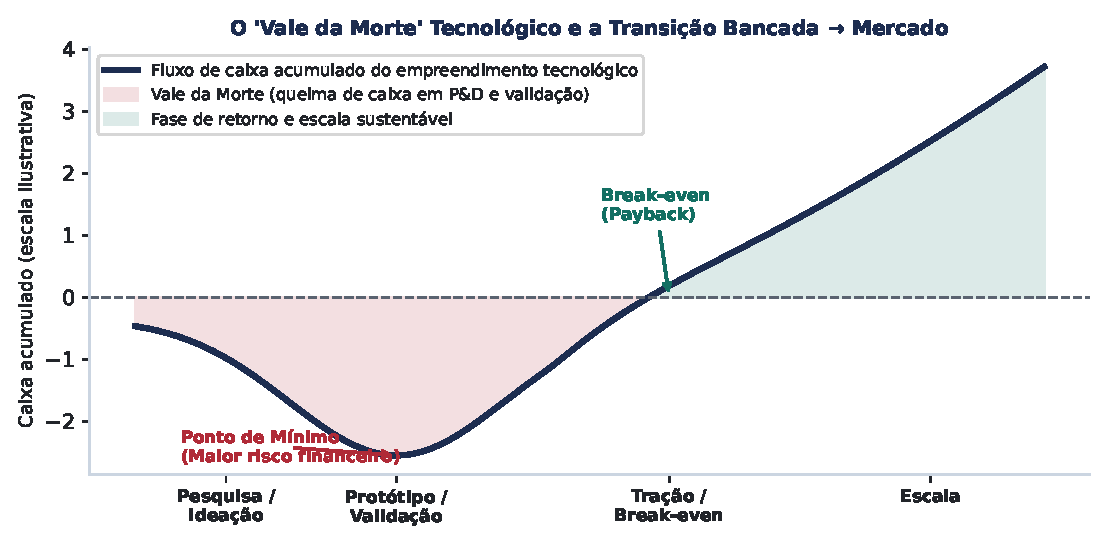
\includegraphics[width=0.90\textwidth]{figures/fig07_vale_da_morte.pdf}
  \caption{Curva J do fluxo de caixa acumulado, Vale da Morte Tecnológico e articulação com a escala de maturidade TRL 1–9.}
  \label{fig:07_vale_morte}
\end{figure}

\begin{boxFormula}[Modelo do Fluxo de Caixa Acumulado e \textit{Payback} no Vale da Morte]
  Considere um empreendimento tecnológico com fluxos de caixa líquidos anuais $FC_t$ para $t = 0, 1, \dots, n$. O fluxo de caixa acumulado no período $t$, denotado por $FCA_t$, é dado pela soma sequencial dos fluxos desde o instante inicial:
  \[
    FCA_t = \sum_{k=0}^{t} FC_k = FCA_{t-1} + FC_t, \quad \text{com } FCA_0 = FC_0.
  \]
  A profundidade máxima do Vale da Morte ($V_{\text{máx}}$) corresponde ao menor valor assumido pelo fluxo acumulado enquanto negativo:
  \[
    V_{\text{máx}} = \min_{t} \{FCA_t\}.
  \]
  O prazo de retorno simples (\textit{payback}) ocorre no intervalo entre o último período $t^*$ em que $FCA_{t^*} < 0$ e o período seguinte $t^* + 1$ em que $FCA_{t^*+1} \ge 0$, sendo interpolado linearmente por:
  \[
    \text{Payback} = t^* + \frac{|FCA_{t^*}|}{FC_{t^*+1}}.
  \]
  Note que a interpolação assume distribuição uniforme das entradas líquidas ao longo do ano $t^*+1$.
\end{boxFormula}

\etapa{4}{Estudos de Caso e Exemplos Resolvidos em 7 Passos}

\begin{boxExemplo}{7.1}{Perda Aceitável e Pássaro na Mão em Biofilme de Palma}
  \passoEnunciado{Uma pesquisadora egressa de mestrado desenvolveu um biofilme comestível à base de mucilagem de palma forrageira para ampliar a vida de prateleira de mangas no Vale do São Francisco. Ela avalia se deve buscar financiamento integral para uma planta piloto antes de testar clientes (\textit{Causation}) ou iniciar por validação enxuta (\textit{Effectuation}).}
  \passoDados{Reserva financeira pessoal disponível: R\$\,18.000,00. Acesso conveniado ao laboratório universitário de alimentos por 6 meses a custo zero de aluguel. Disponibilidade de dedicação: 15 horas semanais, mantendo bolsa de pesquisa de R\$\,3.200,00/mês. Orçamento de planta piloto completa (cenário \textit{Causation}): R\$\,140.000,00. Custo de produzir e testar 30 lotes-piloto com 3 cooperativas locais de fruticultura: R\$\,12.000,00.}
  \passoPedido{Comparar a exposição financeira entre as duas lógicas, calcular a margem de segurança da reserva pessoal sob a lógica efetuacional e identificar os princípios de Sarasvathy mobilizados.}
  \passoMetodo{Aplicação dos princípios \textit{Bird-in-Hand} (meios próprios), \textit{Affordable Loss} (perda aceitável) e \textit{Crazy Quilt} (parceria com cooperativas).}
  \passoContas{
    No cenário \textit{Causation}, o desembolso exigido de R\$\,140.000,00 supera a reserva pessoal em:
    \[
      \text{Déficit de capital} = 140.000,00 - 18.000,00 = \text{R\$\,122.000,00}.
    \]
    Além disso, abandonar a bolsa para dedicação integral sem validação comercial geraria custo de oportunidade de $6 \times 3.200,00 = \text{R\$\,19.200,00}$ no semestre.
    No cenário \textit{Effectuation}, a empreendedora fixa a perda aceitável em R\$\,12.000,00 (insumos para 30 lotes-piloto e análises físico-químicas básicas), preservando uma reserva de segurança de:
    \[
      \text{Reserva preservada} = 18.000,00 - 12.000,00 = \text{R\$\,6.000,00} \quad (33{,}33\% \text{ da reserva}).
    \]
    As 3 cooperativas fornecem as frutas e o espaço de câmara fria para teste em troca de acesso prioritário à tecnologia (pré-compromisso).
  }
  \passoResposta{A abordagem efetuacional reduz a necessidade imediata de capital em 91{,}43\% (de R\$\,140.000,00 para R\$\,12.000,00), preserva R\$\,6.000,00 de reserva e evita R\$\,19.200,00 de perda de renda no semestre inicial.}
  \passoVerificacao{Economicidade e aderência territorial estão preservadas: o laboratório universitário e as cooperativas locais funcionam como amortecedores do risco tecnológico sem endividamento precoce.}
\end{boxExemplo}

\begin{boxExemplo}{7.2}{Mapeamento da Curva J, Vale da Morte e \textit{Payback} em Sensoriamento IoT}
  \passoEnunciado{Uma startup de Feira de Santana desenvolve nós sensores IoT de baixo custo para monitoramento de umidade do solo em perímetros irrigados. O projeto encontra-se em transição do nível TRL 4 para TRL 7.}
  \passoDados{Fluxos de caixa líquidos anuais projetados (em R\$): Ano 0 = $-85.000$; Ano 1 = $-130.000$; Ano 2 = $-45.000$; Ano 3 = $+90.000$; Ano 4 = $+195.000$; Ano 5 = $+260.000$.}
  \passoPedido{Calcular o fluxo de caixa acumulado ano a ano, identificar o ano e o valor do fundo do Vale da Morte e determinar o \textit{payback} simples do projeto.}
  \passoMetodo{Cálculo recursivo de $FCA_t = FCA_{t-1} + FC_t$ e interpolação linear do \textit{payback}.}
  \passoContas{
    Calculando o fluxo acumulado período a período:
    \begin{itemize}[leftmargin=1.4em, itemsep=1pt]
      \item Ano 0: $FCA_0 = -85.000$
      \item Ano 1: $FCA_1 = -85.000 + (-130.000) = -215.000$
      \item Ano 2: $FCA_2 = -215.000 + (-45.000) = -260.000$
      \item Ano 3: $FCA_3 = -260.000 + 90.000 = -170.000$
      \item Ano 4: $FCA_4 = -170.000 + 195.000 = +25.000$
      \item Ano 5: $FCA_5 = +25.000 + 260.000 = +285.000$
    \end{itemize}
    O menor valor acumulado ocorre no Ano 2, com $V_{\text{máx}} = -\text{R\$\,260.000,00}$. Como $FCA_3 = -170.000 < 0$ e $FCA_4 = +25.000 > 0$, o ponto de equilíbrio acumulado ocorre durante o Ano 4 ($t^* = 3$):
    \[
      \text{Payback} = 3 + \frac{|-170.000|}{195.000} = 3 + 0{,}8718 \approx 3{,}87\text{ anos} \quad (\text{cerca de } 46{,}5\text{ meses}).
    \]
  }
  \passoResposta{O fundo do Vale da Morte ocorre no Ano 2, exigindo cobertura acumulada de caixa de R\$\,260.000,00; o \textit{payback} simples é atingido em 3{,}87 anos.}
  \passoVerificacao{O perfil em J é coerente com EBTs de hardware agrícola: os dois primeiros anos concentram prototipagem em campo e homologação (TRL 4–6), e o capital mínimo necessário para não quebrar antes da virada é de pelo menos R\$\,260.000,00.}
\end{boxExemplo}

\begin{boxExemplo}{7.3}{Nexo Indivíduo–Oportunidade na Cadeia do Sisal}
  \passoEnunciado{Dois empreendedores avaliam implantar uma unidade de extração de nanocelulose a partir de resíduos do desfibramento do sisal em Valente (BA). O Empreendedor A é engenheiro químico com 8 anos de atuação técnica em cooperativas sisaleiras; o Empreendedor B é gestor financeiro da capital sem experiência prévia na cadeia agrícola.}
  \passoDados{Acesso a fornecedores de resíduo: A obtém matéria-prima via acordo cooperativo a R\$\,40,00/t; B precisa contratar intermediários a R\$\,110,00/t. Demanda mensal de resíduo: 50 toneladas. Custo mensal de consultoria técnica externa para suprir desconhecimento de processo: R\$\,0,00 para A e R\$\,6.500,00 para B.}
  \passoPedido{Quantificar a vantagem de custo operacional mensal conferida pelo conhecimento prévio e pelas redes territoriais no nexo indivíduo–oportunidade.}
  \passoMetodo{Comparação direta de custos operacionais vinculados à assimetria de informação e conhecimento tácito (Shane \& Venkataraman, 2000).}
  \passoContas{
    Custo mensal com matéria-prima:
    \[
      \text{Custo MP}_A = 50 \times 40{,}00 = \text{R\$\,2.000,00}, \qquad \text{Custo MP}_B = 50 \times 110{,}00 = \text{R\$\,5.500,00}.
    \]
    Somando a consultoria técnica exigida pela ausência de conhecimento prévio:
    \[
      \text{Custo Total}_A = 2.000,00 + 0 = \text{R\$\,2.000,00/mês},
    \]
    \[
      \text{Custo Total}_B = 5.500,00 + 6.500,00 = \text{R\$\,12.000,00/mês}.
    \]
    A diferença mensal é de $12.000,00 - 2.000,00 = \text{R\$\,10.000,00/mês}$ (ou R\$\,120.000,00/ano).
  }
  \passoResposta{O nexo indivíduo–oportunidade enraizado no território gera uma economia operacional de R\$\,10.000,00 mensais para o Empreendedor A.}
  \passoVerificacao{O resultado explica empiricamente por que oportunidades tecnológicas territoriais são mais viáveis quando lideradas por agentes com conhecimento tácito da cadeia local ou em sociedade com eles.}
\end{boxExemplo}

\begin{boxExemplo}{7.4}{Orçamento Escalonado por Níveis de Maturidade TRL 3 a 7}
  \passoEnunciado{Um grupo de pesquisa em biotecnologia ambiental planeja levar um biofertilizante microencapsulado da prova de conceito em bancada (TRL 3) até a demonstração em propriedade agrícola real (TRL 7).}
  \passoDados{Custos estimados por transição de estágio: TRL 3$\to$4 = R\$\,35.000,00; TRL 4$\to$5 = R\$\,65.000,00; TRL 5$\to$6 = R\$\,120.000,00; TRL 6$\to$7 = R\$\,180.000,00. Um edital de subvenção econômica financia 75\% do orçamento total, e investidores-anjo cobrem os 25\% restantes.}
  \passoPedido{Calcular o orçamento total da travessia TRL 3$\to$7, o percentual concentrado na faixa crítica do Vale da Morte (TRL 4$\to$6) e a divisão de fontes de financiamento.}
  \passoMetodo{Soma segmentada por estágio de maturidade tecnológica e rateio proporcional.}
  \passoContas{
    Orçamento total:
    \[
      C_{\text{total}} = 35.000 + 65.000 + 120.000 + 180.000 = \text{R\$\,400.000,00}.
    \]
    Parcela correspondente às transições TRL 4$\to$5 e TRL 5$\to$6:
    \[
      C_{\text{4--6}} = 65.000 + 120.000 = \text{R\$\,185.000,00} \implies \frac{185.000}{400.000} = 0{,}4625 = 46{,}25\%.
    \]
    Parcela da subvenção econômica (75\%) e do investimento-anjo (25\%):
    \[
      \text{Subvenção} = 400.000 \times 0{,}75 = \text{R\$\,300.000,00}, \qquad \text{Anjo} = 400.000 \times 0{,}25 = \text{R\$\,100.000,00}.
    \]
  }
  \passoResposta{O orçamento total é de R\$\,400.000,00, com 46{,}25\% concentrados entre TRL 4 e TRL 6, coberto por R\$\,300.000,00 de subvenção e R\$\,100.000,00 de aporte-anjo.}
  \passoVerificacao{Note que os custos crescem monotonicamente com a escala do ambiente de teste (bancada para campo), justificando a combinação entre recurso público não reembolsável e capital privado paciente.}
\end{boxExemplo}

\begin{boxExemplo}{7.5}{Reconfiguração Efetuacional por Contingência (Princípio da Limonada)}
  \passoEnunciado{Uma startup desenvolveu um filtro cerâmico poroso para dessalinização de água salobra em comunidades rurais do Semiárido. Durante os testes em campo (TRL 6), constatou-se que a vazão obtida era 40\% inferior à necessária para abastecimento humano contínuo, inviabilizando o contrato original com a companhia estadual de saneamento.}
  \passoDados{A mesma cerâmica apresentou retenção de 96\% de corantes têxteis e óleos emulsionados em ensaios paralelos. Custo já investido (afundado): R\$\,90.000,00. Custo adicional para adaptar o módulo ao tratamento de efluentes de pequenas lavanderias industriais da região: R\$\,25.000,00. Receita anual potencial em 15 lavanderias locais: R\$\,11.000,00/lavanderia.}
  \passoPedido{Avaliar a decisão segundo o princípio da Limonada (\textit{Effectuation}) e calcular o retorno incremental sobre o novo aporte necessário.}
  \passoMetodo{Desconsideração de custos afundados (\textit{sunk costs}), reorientação estratégica pela contingência e cálculo de receita potencial incremental.}
  \passoContas{
    Os R\$\,90.000,00 já gastos constituem custo afundado e não devem condicionar a decisão futura. O investimento incremental exigido para pivotar para o mercado de efluentes têxteis é de R\$\,25.000,00. A receita bruta anual potencial com as 15 lavanderias regionais é:
    \[
      R_{\text{anual}} = 15 \times 11.000,00 = \text{R\$\,165.000,00/ano}.
    \]
    Comparando a receita anual potencial com o aporte incremental de adaptação:
    \[
      \frac{165.000}{25.000} = 6{,}6\text{ vezes o capital incremental necessário para a adaptação}.
    \]
  }
  \passoResposta{Aplicando o princípio da Limonada, a equipe aproveita a propriedade filtrante descoberta na falha de vazão para abrir um mercado industrial regional de R\$\,165.000,00/ano com aporte incremental de R\$\,25.000,00.}
  \passoVerificacao{A decisão evita o abandono prematuro do ativo tecnológico e demonstra como o diálogo com demandas produtivas do território transforma limitações técnicas em novos modelos de negócio.}
\end{boxExemplo}

\etapa{5}{Armadilhas Conceituais e Erros Mais Comuns}

\begin{boxErro}[Erro 1 — Confundir \textit{Effectuation} com Improvisação sem Método]
  Assumir que a lógica efetuacional dispensa disciplina analítica, registros financeiros ou metas verificáveis é um equívoco recorrente. Na realidade, o \textit{Effectuation} substitui a previsão de longo prazo pela experimentação controlada com perda aceitável (\textit{affordable loss}) e compromissos formais com parceiros. Improvisar sem definir o limite de perda leva à exaustão de caixa.
\end{boxErro}

\begin{boxErro}[Erro 2 — Subestimar o Custo da Transição TRL 4 para TRL 7]
  Muitos pesquisadores tratam a obtenção de um protótipo funcional em bancada (TRL 4) como sinônimo de produto pronto para venda. Na prática, certificação regulatória, engenharia de manufatura, embalagem, logística e assistência técnica em ambiente operacional costumam custar de três a dez vezes mais do que a pesquisa inicial de laboratório.
\end{boxErro}

\begin{boxErro}[Erro 3 — Ignorar o Fluxo Acumulado ao Analisar o Vale da Morte]
  Avaliar apenas o resultado positivo de um ano futuro (por exemplo, $+90.000$ no Ano 3) sem somar os déficits acumulados dos anos anteriores induz à falsa impressão de suficiência de caixa. Se o fundo do Vale da Morte exige R\$\,260.000,00 acumulados, o projeto quebrará no Ano 2 mesmo que o Ano 3 seja superavitário.
\end{boxErro}

\begin{boxErro}[Erro 4 — Aplicar Lógica \textit{Causation} Rígida em Mercados Inexistentes]
  Exigir projeções econométricas de cinco anos para uma tecnologia radical sem precedentes de consumo gera apenas ficção numérica. Quando não há série histórica confiável, o uso prematuro de planos rígidos imobiliza capital em premissas não testadas em vez de financiar ciclos curtos de aprendizado.
\end{boxErro}

\etapa{6}{Lista de Exercícios (15 Questões em 3 Níveis)}

\textbf{Nível 1 — Fundamentos Conceituais (Questões 1 a 5)}

\begin{enumerate}[leftmargin=1.5em, itemsep=6pt]
  \item Explique, com base em Shane e Venkataraman (2000), por que a existência de uma nova tecnologia em uma universidade não gera automaticamente um empreendimento sem a mediação do nexo indivíduo–oportunidade.
  \espacoResolucao[1.8cm]

  \item Diferencie os critérios de tomada de decisão das lógicas \textit{Causation} e \textit{Effectuation} quanto ao ponto de partida, à postura diante do risco e ao relacionamento com outros atores do mercado.
  \espacoResolucao[1.8cm]

  \item Associe cada um dos cinco princípios de Sarasvathy (pássaro na mão, perda aceitável, colcha de retalhos, limonada e piloto no avião) a uma ação prática de um grupo de pós-graduandos iniciando uma startup territorial.
  \espacoResolucao[2.0cm]

  \item Descreva o que caracteriza os níveis TRL 3, TRL 6 e TRL 9 e explique por que o Vale da Morte Tecnológico concentra-se tipicamente entre TRL 4 e TRL 6.
  \espacoResolucao[1.8cm]

  \item Por que o fluxo de caixa acumulado descreve uma Curva em J nos empreendimentos de base tecnológica? Indique o significado econômico do ponto mínimo da curva e do cruzamento do eixo horizontal.
  \espacoResolucao[1.8cm]

  \item \textbf{(Nível 2 — Aplicações Numéricas)} Uma startup de biotecnologia apresenta os seguintes fluxos de caixa líquidos anuais (em R\$): Ano 0 = $-60.000$; Ano 1 = $-90.000$; Ano 2 = $-30.000$; Ano 3 = $+75.000$; Ano 4 = $+150.000$. Calcule o fluxo de caixa acumulado para cada ano, o valor do fundo do Vale da Morte e o \textit{payback} simples.
  \espacoResolucao[2.4cm]

  \item Uma empreendedora possui R\$\,25.000,00 de reserva pessoal e define como perda aceitável exatamente 40\% desse valor para validar um aplicativo de rastreabilidade agrícola em 4 meses. Caso o experimento falhe, qual será o valor perdido e qual a reserva preservada? Se o custo de um desenvolvedor terceirizado fosse R\$\,18.000,00, o projeto caberia na perda aceitável?
  \espacoResolucao[2.2cm]

  \item Um projeto de equipamento agroindustrial estima custos de R\$\,40.000,00 (TRL 3$\to$4), R\$\,80.000,00 (TRL 4$\to$5), R\$\,130.000,00 (TRL 5$\to$6) e R\$\,250.000,00 (TRL 6$\to$7). Calcule o orçamento total e a participação percentual da etapa TRL 6$\to$7 no total necessário.
  \espacoResolucao[2.2cm]

  \item Dois projetos concorrem a um fundo territorial. O Projeto Alfa segue lógica \textit{Causation} e exige R\$\,320.000,00 iniciais para montar fábrica antes das vendas. O Projeto Beta usa \textit{Effectuation}, firmando pré-compromisso com uma cooperativa que cede galpão e reduz o investimento inicial em 62{,}5\%. Qual o aporte inicial necessário para o Projeto Beta?
  \espacoResolucao[2.2cm]

  \item Uma equipe obteve fluxo de caixa acumulado de $-\text{R\$\,180.000,00}$ ao final do Ano 2. Nos Anos 3 e 4, os fluxos líquidos positivos são de R\$\,100.000,00 e R\$\,160.000,00, respectivamente. Em quantos anos ocorre o \textit{payback} simples?
  \espacoResolucao[2.2cm]

  \item \textbf{(Nível 3 — Análise Territorial e Estratégica)} Analise como a presença de uma universidade estadual e de cooperativas agrícolas em um território semiárido altera os princípios "pássaro na mão" e "colcha de retalhos" para um pesquisador local em comparação a um empreendedor isolado em região sem infraestrutura de CT\&I.
  \espacoResolucao[2.2cm]

  \item Um projeto de dessalinização solar apresenta $FC_0 = -100.000$, $FC_1 = -140.000$, $FC_2 = +60.000$, $FC_3 = +120.000$ e $FC_4 = +150.000$. Caso um edital de subvenção econômica cubra R\$\,120.000,00 no Ano 1 (reduzindo o déficit do Ano 1 para $-20.000$), em quanto diminui a profundidade do Vale da Morte e qual passa a ser o novo \textit{payback} simples?
  \espacoResolucao[2.5cm]

  \item Discuta em que momento do ciclo de vida de uma EBT a equipe deve migrar da predominância de \textit{Effectuation} para a incorporação sistemática de ferramentas de \textit{Causation}, justificando os riscos de realizar essa transição cedo demais ou tarde demais.
  \espacoResolucao[2.2cm]

  \item Uma pesquisadora gastou R\$\,50.000,00 desenvolvendo um sensor para o setor petrolífero, mas o cliente cancelou o projeto por mudança regulatória. Para adaptar o sensor ao monitoramento de barragens de rejeitos minerais na Bahia, são necessários R\$\,30.000,00 adicionais, com receita líquida estimada de R\$\,45.000,00/ano durante 3 anos. Desconsiderando custos afundados, a adaptação é atrativa? Justifique quantitativamente.
  \espacoResolucao[2.4cm]

  \item Elabore uma matriz comparativa indicando como três falhas típicas no Vale da Morte (ausência de validação com usuário, falta de capital paciente e subestimação de certificação) podem ser mitigadas articulando \textit{Effectuation} e instrumentos territoriais de fomento.
  \espacoResolucao[2.4cm]
\end{enumerate}

\etapa{7}{Questões Autorais Estilo Pós-Graduação / Concursos de CT\&I}

\begin{enumerate}[leftmargin=1.5em, itemsep=6pt]
  \item \textbf{(Estilo ANPAD / Gestão da Inovação)} Considere as assertivas sobre o processo empreendedor segundo Shane \& Venkataraman (2000) e Sarasvathy (2001):
  I. O nexo indivíduo–oportunidade sustenta que oportunidades empreendedoras são percebidas igualmente por todos os agentes econômicos que têm acesso à mesma informação pública.
  II. Na lógica \textit{Effectuation}, o princípio da perda aceitável substitui o cálculo do retorno máximo esperado como critério de decisão em ambientes de incerteza knightiana.
  III. A lógica \textit{Causation} é inadequada para qualquer etapa de uma empresa, devendo ser abandonada mesmo após a consolidação do mercado.
  Assinale a alternativa correta:
  \begin{alternativas}
    \item Apenas I está correta.
    \item Apenas II está correta.
    \item Apenas I e II estão corretas.
    \item Apenas II e III estão corretas.
    \item I, II e III estão corretas.
  \end{alternativas}
  \espacoResolucao[1.5cm]

  \item \textbf{(Estilo Concurso Analista de CT\&I — FINEP/FAPs)} Uma empresa de base tecnológica apresenta os fluxos de caixa líquidos anuais (em milhares de R\$): Ano 0 = $-120$; Ano 1 = $-180$; Ano 2 = $-60$; Ano 3 = $+150$; Ano 4 = $+210$; Ano 5 = $+240$. Sobre o perfil da Curva J desse empreendimento, assinale a alternativa correta:
  \begin{alternativas}
    \item O fundo do Vale da Morte ocorre no Ano 1, com déficit acumulado de R\$\,300 mil.
    \item O fundo do Vale da Morte ocorre no Ano 2, com déficit acumulado de R\$\,360 mil, e o \textit{payback} simples ocorre exatamente ao final do Ano 4.
    \item O fundo do Vale da Morte ocorre no Ano 2, com déficit acumulado de R\$\,360 mil, e o \textit{payback} simples ocorre entre o Ano 3 e o Ano 4.
    \item O \textit{payback} simples ocorre aos 3{,}50 anos.
    \item O projeto nunca atinge saldo acumulado positivo até o Ano 5.
  \end{alternativas}
  \espacoResolucao[1.6cm]

  \item \textbf{(Estilo Discursiva de Seleção de Mestrado / PPGPT)} Analise criticamente a seguinte afirmação: ``O Vale da Morte Tecnológico resulta exclusivamente da escassez de crédito bancário comercial nos países em desenvolvimento''. Em sua resposta, articule os conceitos de maturidade tecnológica (TRL), incerteza knightiana e o papel das alianças efetuacionais (\textit{crazy quilt}) na superação dessa fase.
  \espacoResolucao[2.5cm]
\end{enumerate}

\begin{boxDica}[Contraponto Crítico e Prática Territorial (AV3)]
  Ao estruturar o seu Projeto Final (AV3), evite apresentar um plano de negócios puramente preditivo se a tecnologia ou o arranjo territorial ainda estiver em fase de validação (TRL 3–5). Explicite quais são os seus meios atuais (\textit{Bird-in-Hand}), qual é a perda aceitável para o primeiro ciclo de testes e quais cooperativas, laboratórios ou prefeituras compõem a sua colcha de retalhos (\textit{Crazy Quilt}).
\end{boxDica}

\clearpage
\etapa{8}{Gabarito Integralmente Comentado (Exercícios 1 a 18)}

\begin{boxGabarito}[Resolução Completa dos Exercícios da Etapa 6 (1 a 15) e Etapa 7 (16 a 18)]
  \begin{enumerate}[leftmargin=1.5em, itemsep=4pt]
    \item \textbf{Resposta:} Segundo Shane e Venkataraman (2000), a oportunidade tecnológica objetiva precisa ser percebida, avaliada e explorada por um indivíduo ou equipe dotado de conhecimento prévio e capacidade cognitiva para conectar a solução técnica a uma demanda real. Sem esse nexo, a patente ou protótipo permanece ocioso na bancada.
    \item \textbf{Resposta:} \textit{Causation} parte de uma meta fixa, decide pela maximização do retorno esperado e vê outros atores principalmente como concorrentes a analisar. \textit{Effectuation} parte dos meios disponíveis, decide pela perda aceitável e busca parcerias de pré-compromisso para co-criar o mercado.
    \item \textbf{Resposta:} \textit{Pássaro na mão}: mapear competências do grupo, equipamentos do laboratório e contatos locais; \textit{Perda aceitável}: limitar gastos iniciais a uma reserva definida; \textit{Colcha de retalhos}: envolver cooperativa ou prefeitura como parceira de teste; \textit{Limonada}: adaptar o produto caso o teste revele uso alternativo; \textit{Piloto no avião}: conduzir negociações ativas em vez de esperar tendências externas.
    \item \textbf{Resposta:} TRL 3 representa a prova de conceito experimental em laboratório; TRL 6, a demonstração de protótipo em ambiente relevante real; TRL 9, o sistema operando comercialmente. Entre TRL 4 e 6 ocorre o Vale da Morte porque os editais de pesquisa básica já terminaram e o capital privado ainda exige comprovação comercial para investir.
    \item \textbf{Resposta:} A curva tem formato de J porque os desembolsos iniciais em P\&D, prototipagem e certificação geram fluxos líquidos negativos antes das vendas recorrentes. O ponto mínimo indica a necessidade máxima de capital acumulado para atravessar o Vale da Morte; o cruzamento do eixo horizontal indica o \textit{payback} simples (recuperação do capital investido).
    \item \textbf{Resposta:} $FCA_0 = -60.000$; $FCA_1 = -60.000 - 90.000 = -150.000$; $FCA_2 = -150.000 - 30.000 = -180.000$ (fundo do Vale da Morte); $FCA_3 = -180.000 + 75.000 = -105.000$; $FCA_4 = -105.000 + 150.000 = +45.000$. O \textit{payback} ocorre no Ano 4: $3 + 105.000 / 150.000 = 3 + 0{,}70 = 3{,}70\text{ anos}$.
    \item \textbf{Resposta:} Perda aceitável = $25.000 \times 0{,}40 = \text{R\$\,10.000,00}$. Reserva preservada = $25.000 - 10.000 = \text{R\$\,15.000,00}$. A contratação de R\$\,18.000,00 excederia a perda aceitável em R\$\,8.000,00, não devendo ser realizada nessa configuração.
    \item \textbf{Resposta:} Orçamento total = $40.000 + 80.000 + 130.000 + 250.000 = \text{R\$\,500.000,00}$. Participação de TRL 6$\to$7 = $250.000 / 500.000 = 0{,}50 = 50\%$.
    \item \textbf{Resposta:} Redução = $320.000 \times 0{,}625 = \text{R\$\,200.000,00}$. Aporte inicial necessário para Beta = $320.000 - 200.000 = \text{R\$\,120.000,00}$.
    \item \textbf{Resposta:} Ao fim do Ano 2, $FCA_2 = -180.000$. No Ano 3, $FCA_3 = -180.000 + 100.000 = -80.000$. No Ano 4, $FCA_4 = -80.000 + 160.000 = +80.000$. Logo, $\text{Payback} = 3 + 80.000 / 160.000 = 3{,}50\text{ anos}$.
    \item \textbf{Resposta:} A universidade amplia o "pássaro na mão" (acesso a laboratórios, orientação científica e bolsistas) e as cooperativas viabilizam a "colcha de retalhos" (espaços de teste, matéria-prima e primeiros usuários), reduzindo o custo de experimentação frente a um empreendedor isolado.
    \item \textbf{Resposta:} Cenário original: $FCA_0 = -100.000$; $FCA_1 = -240.000$ (fundo); $FCA_2 = -180.000$; $FCA_3 = -60.000$; $FCA_4 = +90.000$. Payback original = $3 + 60.000 / 150.000 = 3{,}40\text{ anos}$. Com subvenção de R\$\,120.000 no Ano 1 ($FC_1 = -20.000$): $FCA_0 = -100.000$; $FCA_1 = -120.000$ (novo fundo); $FCA_2 = -60.000$; $FCA_3 = +60.000$. A profundidade do Vale da Morte cai em R\$\,120.000,00 (de R\$\,240.000 para R\$\,120.000, redução de 50\%), e o novo \textit{payback} cai para $2 + 60.000 / 120.000 = 2{,}50\text{ anos}$.
    \item \textbf{Resposta:} A transição deve ocorrer após a validação do problema, da solução e dos primeiros clientes pagantes (TRL 6–7). Migrar cedo demais para \textit{Causation} engessa o negócio em premissas falsas; migrar tarde demais impede a captação de crédito estruturado e a gestão de escala.
    \item \textbf{Resposta:} Sim. Os R\$\,50.000,00 iniciais são custo afundado. O investimento incremental é de R\$\,30.000,00 para gerar R\$\,45.000,00/ano $\times$ 3 anos = R\$\,135.000,00 de receita líquida acumulada, gerando saldo incremental positivo de R\$\,105.000,00 e retorno do aporte adicional em $30.000 / 45.000 \approx 0{,}67\text{ ano}$ (8 meses).
    \item \textbf{Resposta:} (1) Ausência de validação $\to$ mitigada com testes rápidos e pré-compromissos com usuários locais (\textit{Crazy Quilt}); (2) Falta de capital paciente $\to$ mitigada por subvenções estaduais/federais combinadas com perda aceitável; (3) Subestimação de certificação $\to$ mitigada por parcerias com laboratórios credenciados de ICTs desde TRL 4.
    \item \textbf{Questão 16 (Etapa 7) — Gabarito: (B).} I é falsa porque o conhecimento prévio é assimétrico, logo nem todos percebem a mesma oportunidade. II é verdadeira. III é falsa porque \textit{Causation} é útil na fase de escala e previsibilidade.
    \item \textbf{Questão 17 (Etapa 7) — Gabarito: (B).} $FCA_0 = -120$; $FCA_1 = -300$; $FCA_2 = -360$ (fundo do Vale da Morte); $FCA_3 = -210$; $FCA_4 = -210 + 210 = 0$. Logo, o \textit{payback} simples ocorre exatamente ao final do Ano 4 ($4{,}00$ anos).
    \item \textbf{Questão 18 (Etapa 7) — Espelho Discursivo:} A resposta deve refutar o reducionismo creditício, explicando que entre TRL 4 e 6 há elevada incerteza tecnológica e de mercado (incerteza knightiana), que impede a precificação tradicional de risco por bancos comerciais. Deve ainda demonstrar como editais de subvenção e alianças efetuacionais (\textit{crazy quilt}) com usuários-piloto compartilham o risco nessa travessia.
  \end{enumerate}
\end{boxGabarito}

\begin{boxResumo}
  \begin{itemize}[leftmargin=1.4em, itemsep=2pt]
    \item O empreendedorismo emerge do nexo entre indivíduos com conhecimento prévio/redes territoriais e oportunidades econômicas ou socioambientais.
    \item Sob incerteza radical, a lógica \textit{Effectuation} (pássaro na mão, perda aceitável, colcha de retalhos, limonada, piloto no avião) preserva caixa e acelera o aprendizado.
    \item A transição bancada–mercado forma uma Curva J cujo ponto mínimo define o Vale da Morte Tecnológico (TRL 4–6), exigindo planejamento de caixa acumulado e instrumentos híbridos de fomento.
  \end{itemize}
\end{boxResumo}

\begin{boxTeste}
  \begin{enumerate}[leftmargin=1.5em, itemsep=4pt]
    \item (\V/\F) Na lógica \textit{Effectuation}, o empreendedor fixa primeiro uma meta de participação de mercado em cinco anos e depois busca o capital total necessário para atingi-la.
    \item (\V/\F) O princípio da perda aceitável recomenda limitar o investimento experimental ao montante máximo que o empreendedor pode perder sem comprometer sua sobrevivência.
    \item (\V/\F) Um projeto com $FC_0 = -50.000$, $FC_1 = -70.000$ e $FC_2 = +120.000$ apresenta fundo do Vale da Morte de $-\text{R\$\,120.000,00}$ no Ano 1 e atinge \textit{payback} simples exatamente ao final do Ano 2.
    \item (\V/\F) Na escala TRL, o nível 3 corresponde à operação comercial plena em escala industrial.
  \end{enumerate}
  \begin{boxGabarito}[Respostas do Checkpoint — Capítulo 7]
    \textbf{1: \F} (Essa é a lógica \textit{Causation}). \quad \textbf{2: \V}. \quad \textbf{3: \V} ($FCA_1 = -120.000$; $FCA_2 = 0$). \quad \textbf{4: \F} (Operação comercial plena é TRL 9; TRL 3 é prova de conceito em laboratório).
  \end{boxGabarito}
\end{boxTeste}
